\section{Materials}\label{sec:materials}
		The are few materials needed to perform the braketests, most of the materials needed for the validation tests were borrowed from the \textit{Wear of Materials Laboratory} from \textit{University of Brasília}, the way the materials are disposed can been seen in Figure \ref{fig:materials-scheme}.

		\begin{figure}[htbp]
			\centering
			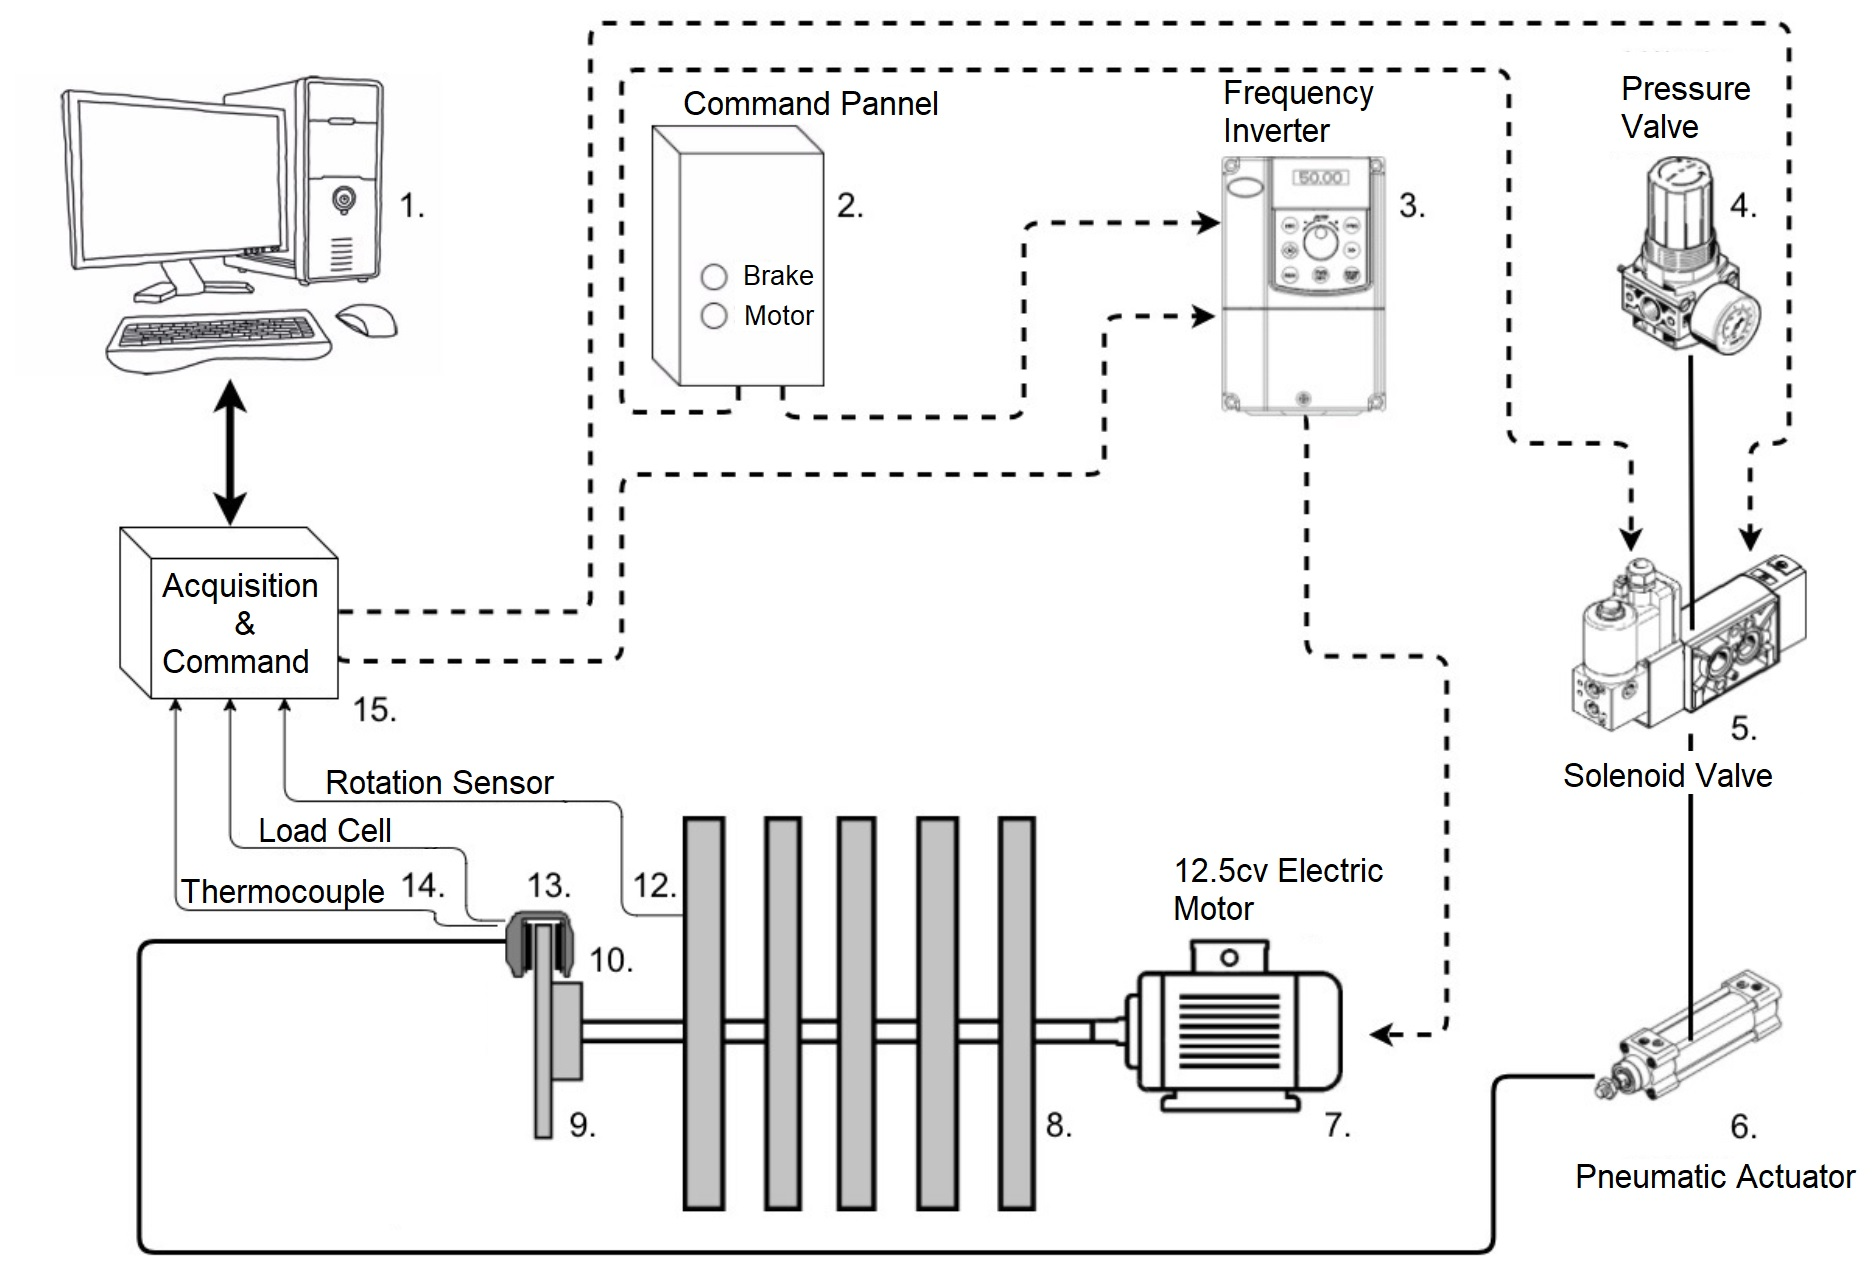
\includegraphics[width=1\textwidth]{figuras/fig-materials-scheme}
			\caption{Materials Disposition}
			\label{fig:materials-scheme}
		\end{figure}

		\par
		The frequency inverter used on the tests is the WEG-CFW08, it is a important part of the tests as it is responsible for controlling the speed and acceleration of the motor by varying the current on the three-phase lines that feeds the motor. It has four digital inputs, two analog inputs, two digital outputs alongside with two analog outputs \cite{wegCFW08Manual}. For the tests only the digital inputs will be used to turn the motor on and off, Figure \ref{fig:frequency-inverter} shows the device installed and fixed on the Laboratory`s pannel.

		\begin{figure}[htbp]
			\centering
			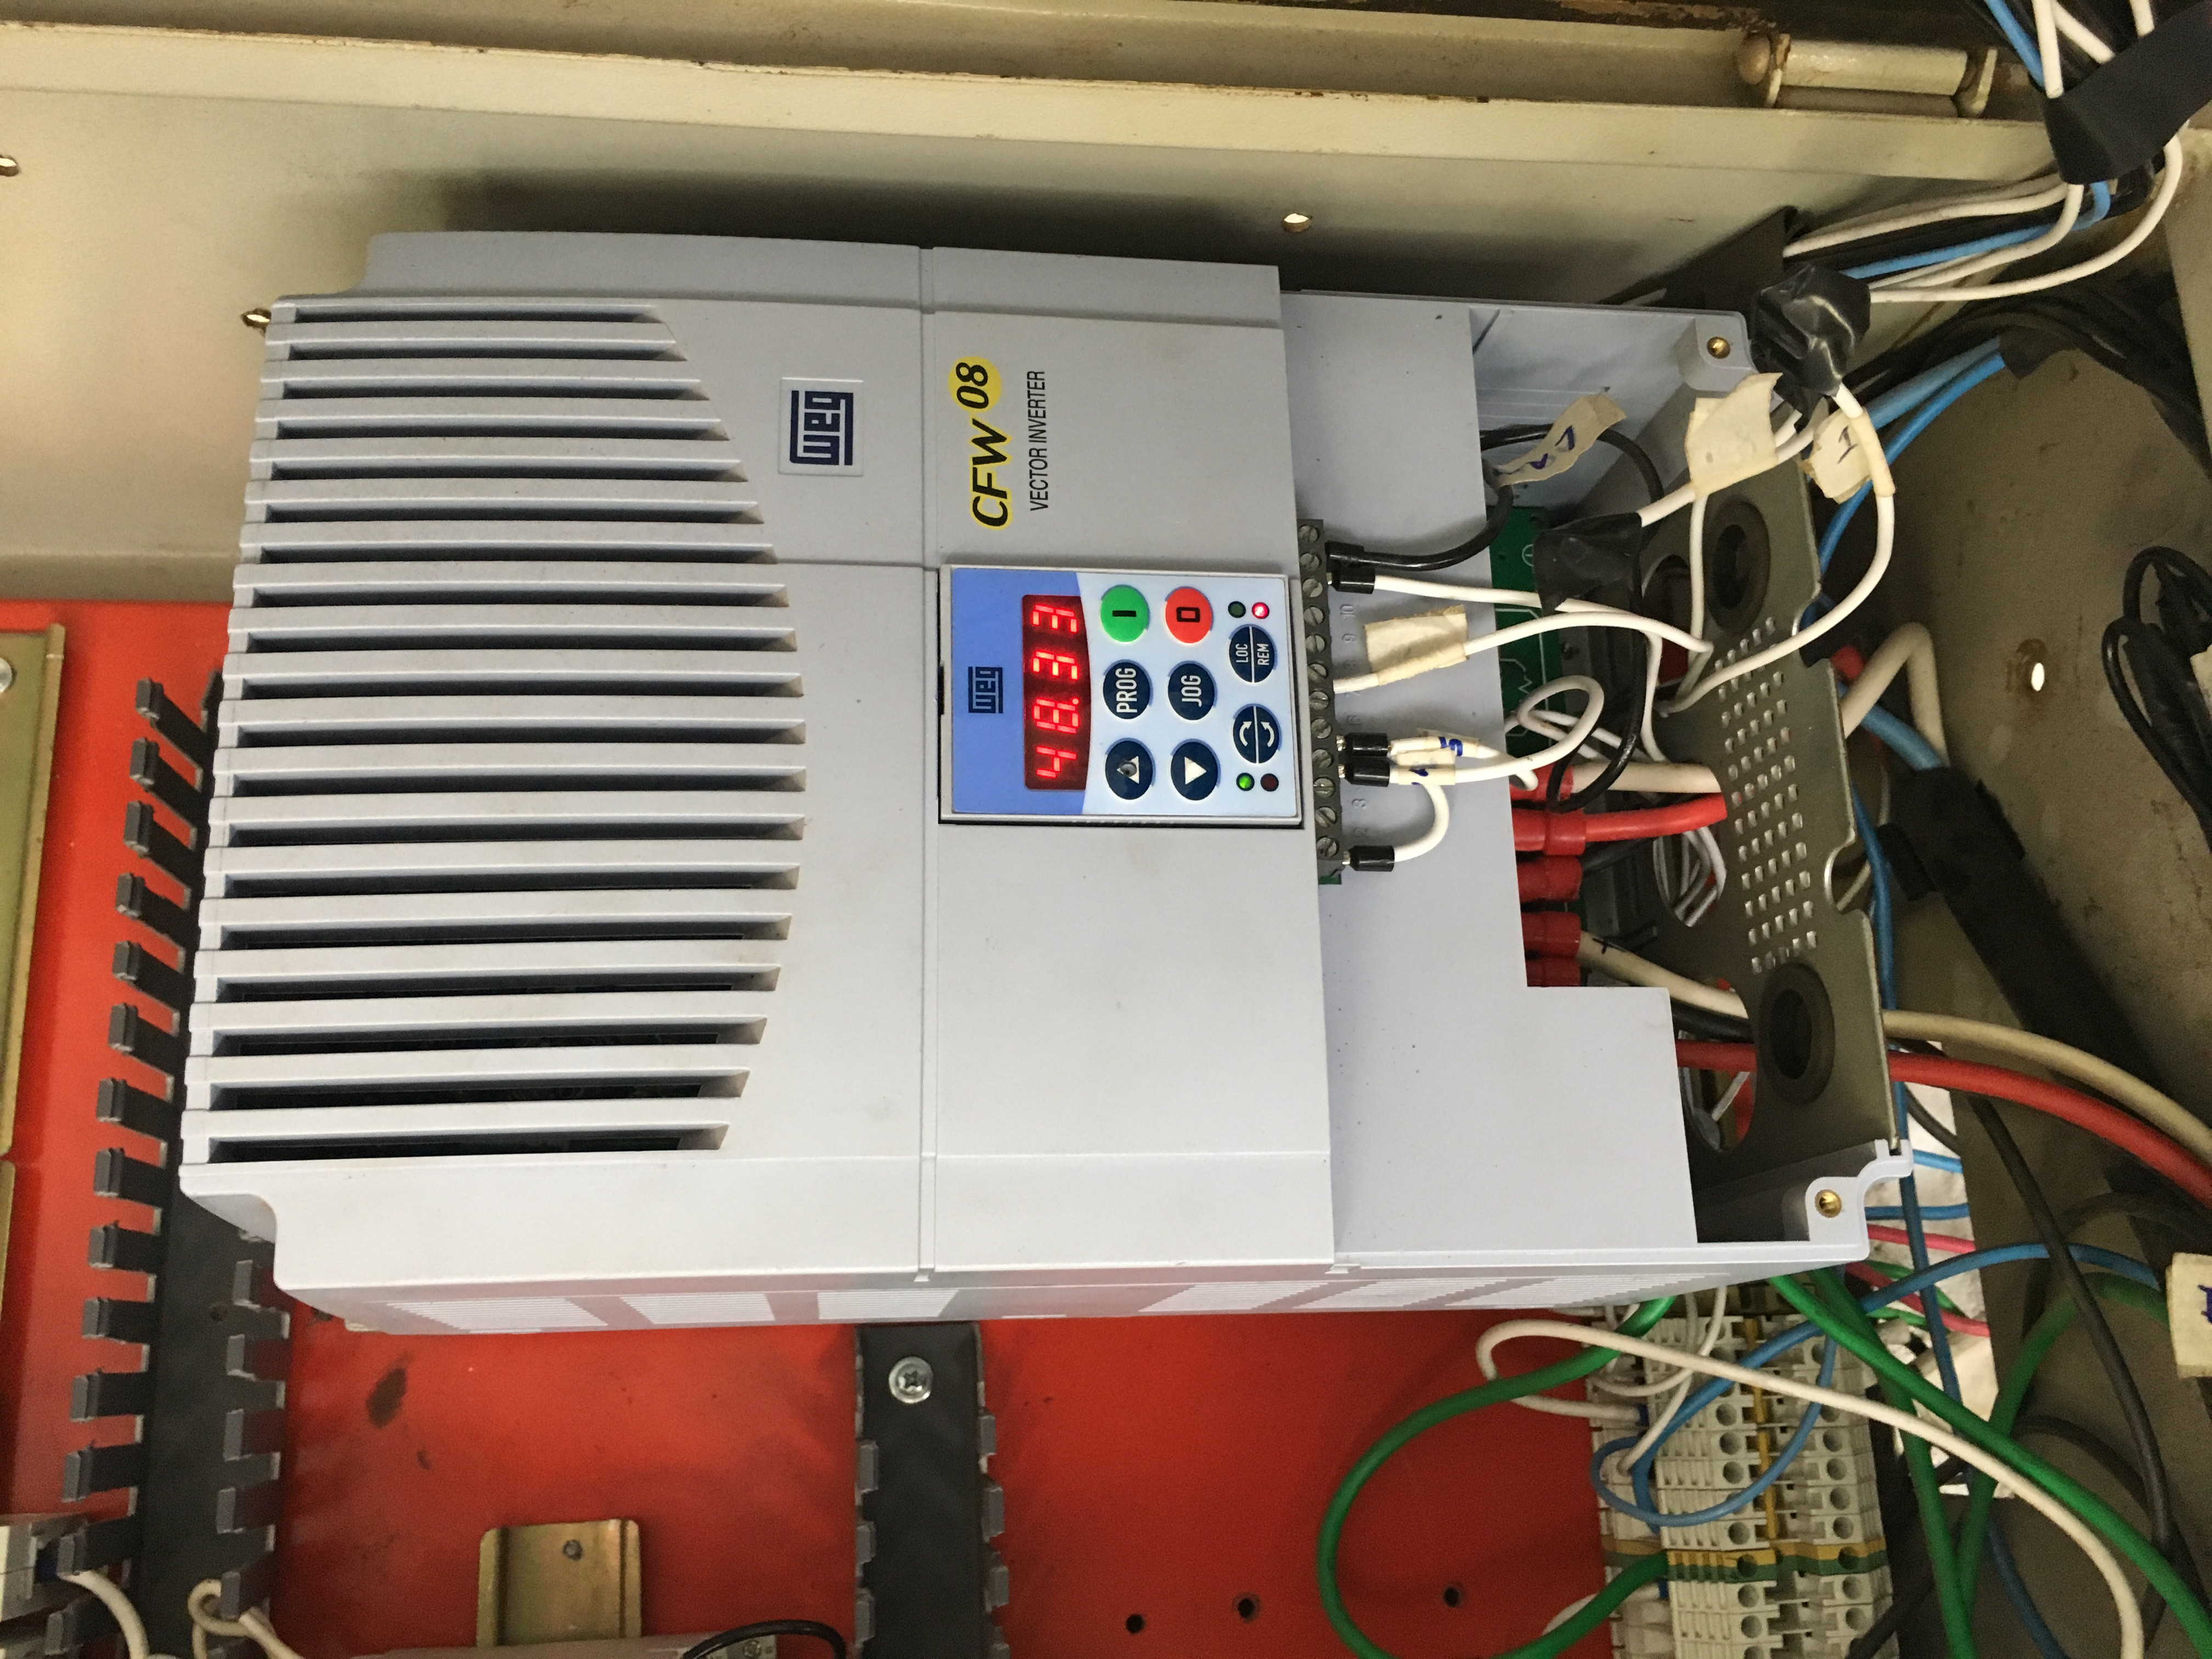
\includegraphics[width=.5\textwidth, angle=270]{figuras/fig-frequency-inverter}
			\caption{Frequency Inverter WEG-CFW08}
			\label{fig:frequency-inverter}
		\end{figure}
		\par

		The electric motor used is manufactured by WEG, this is a three-phase motor that has 12.5 cv of power, 1755 max RPM and has a efficiency of 87.7$\%$ and it is connected to the brake disc machine through a pulley system. Figure \ref{fig:electric-motor} the motor itself.

		\begin{figure}[htbp]
			\centering
			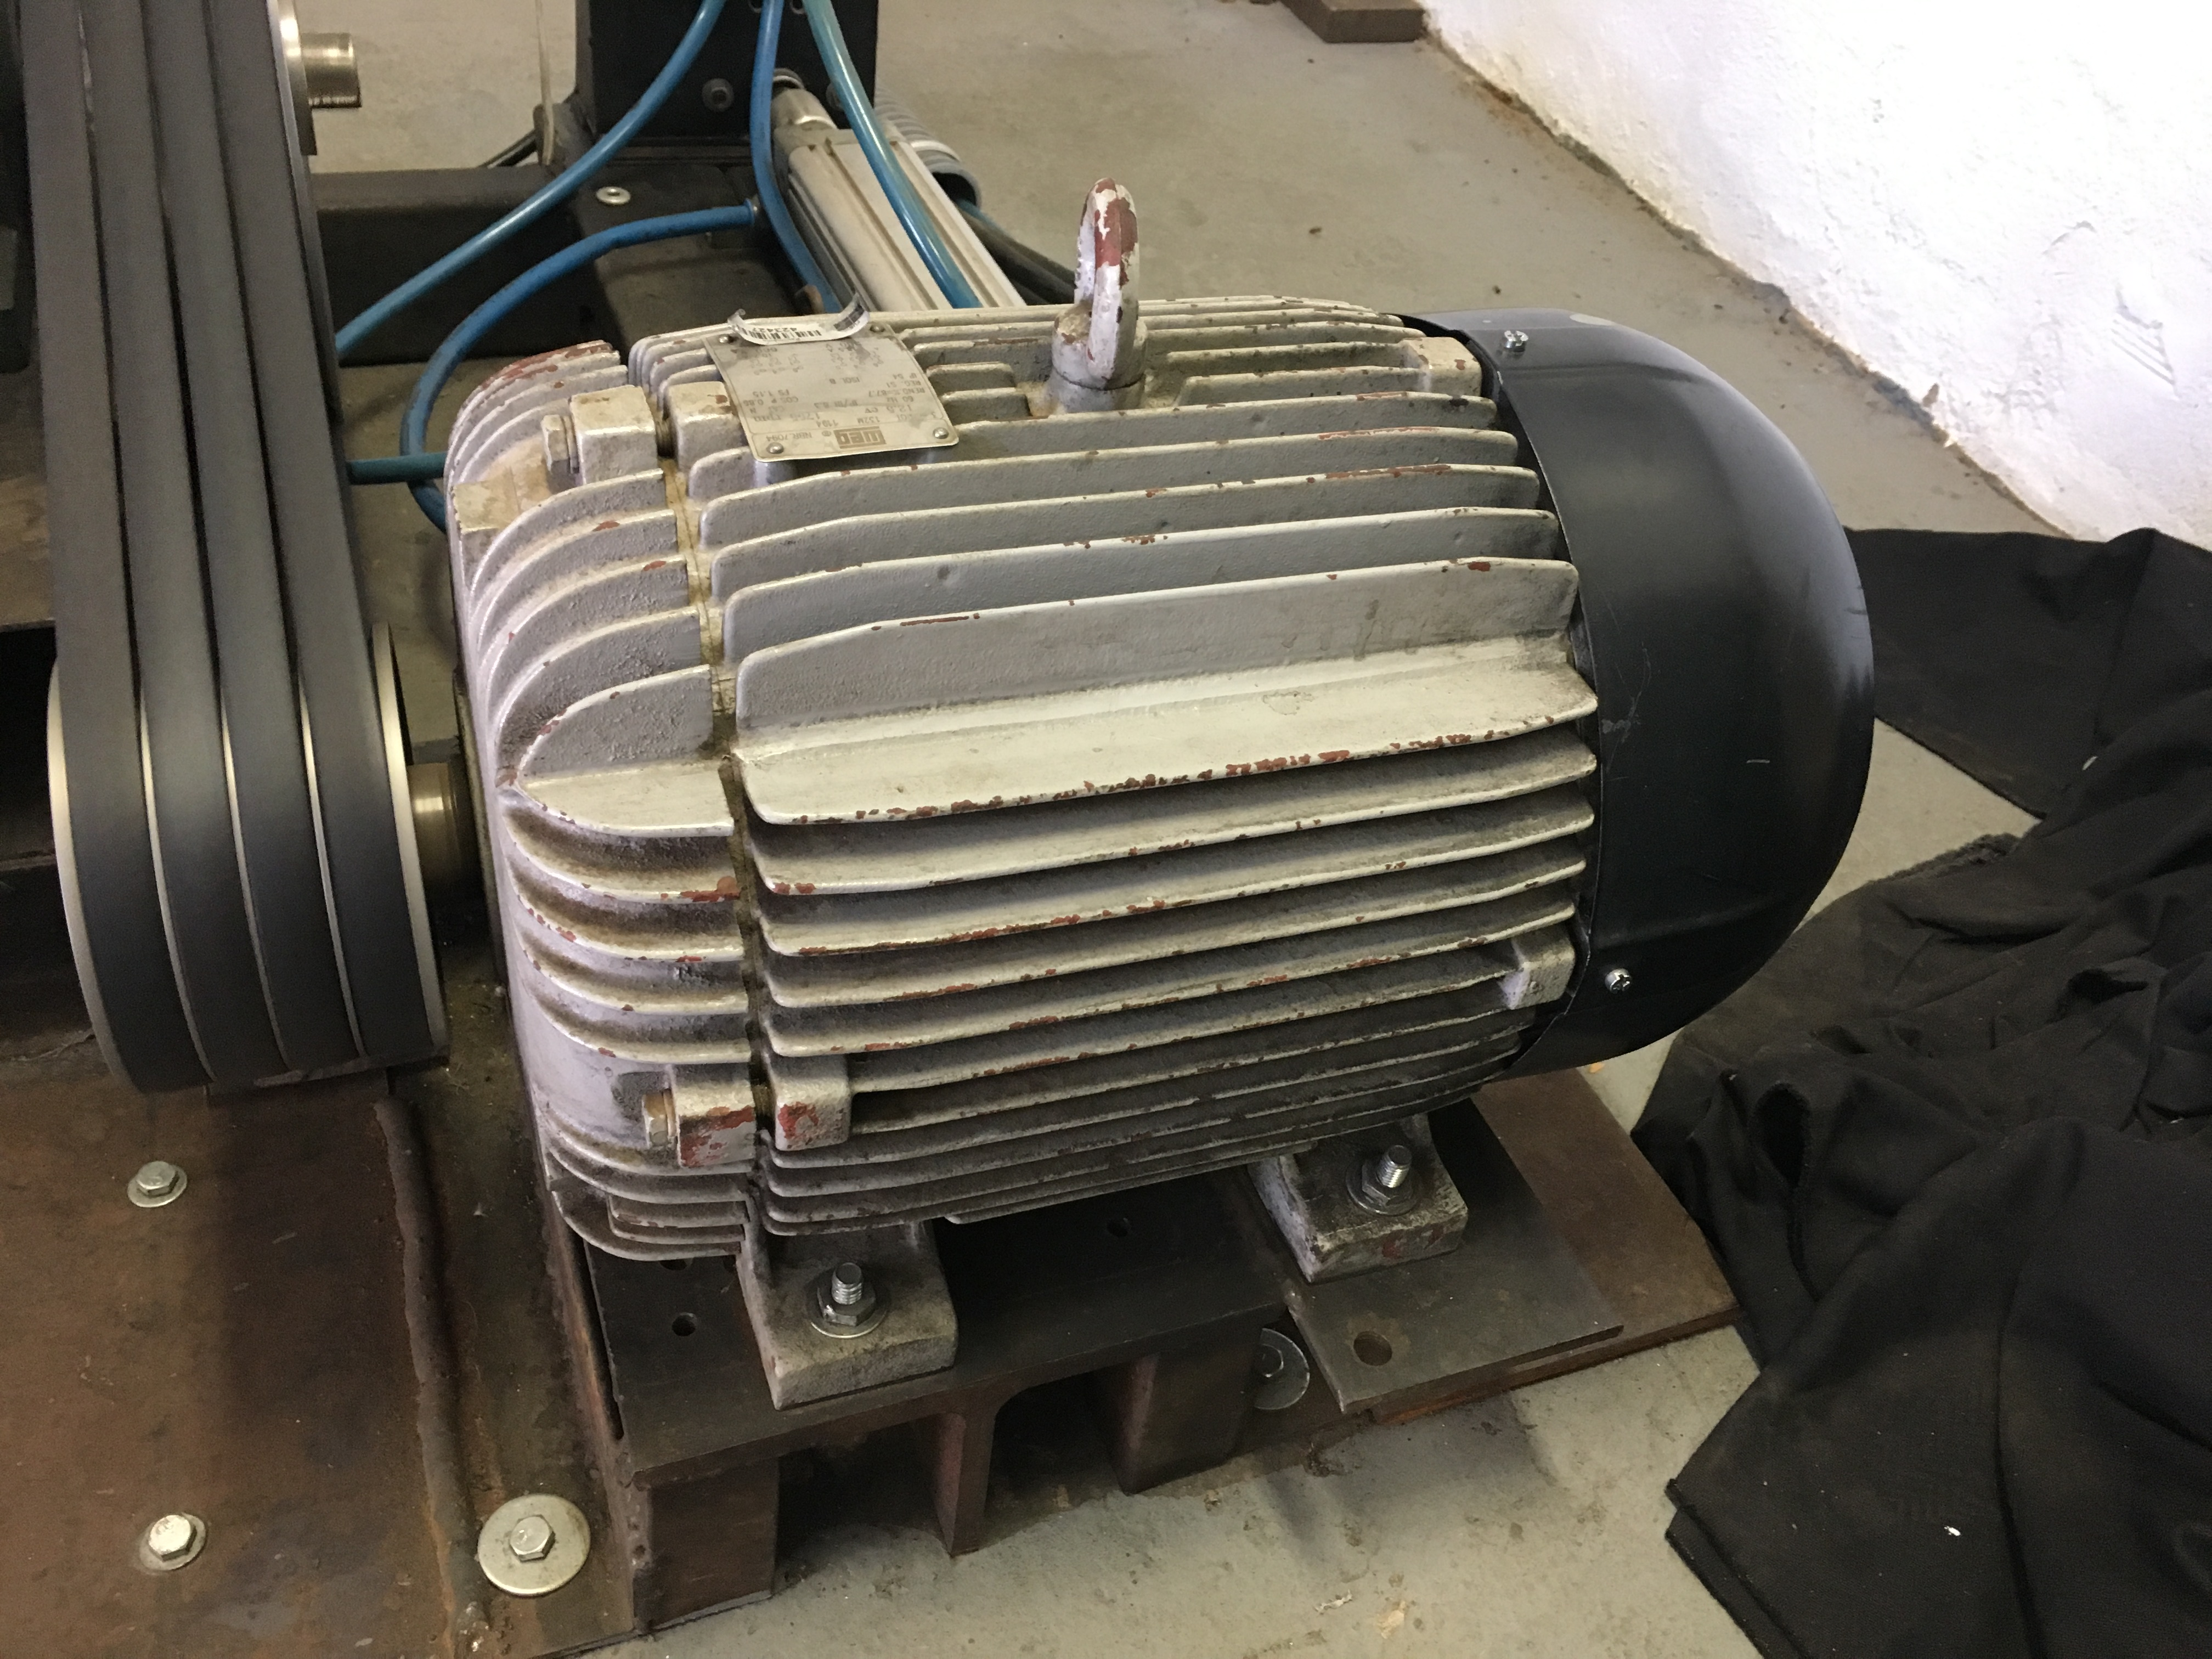
\includegraphics[width=.5\textwidth]{figuras/fig-electric-motor}
			\caption{Electric Motor WEG}
			\label{fig:electric-motor}
		\end{figure}
		\par

		Brake Disc Machine is a machine wielded on \textit{Wear of Materials Laboratory} in order to simulate a car's axle submitted to inertial masses. One end of the axle is connected to the electric motor through a pulley system and the other end is connected to the disc brake components as Figures \ref{fig:brake-disc-machine}, \ref{fig:brake-disc-machine-pulley} and \ref{fig:brake-disc}.

		\begin{figure}[htbp]
			\centering
			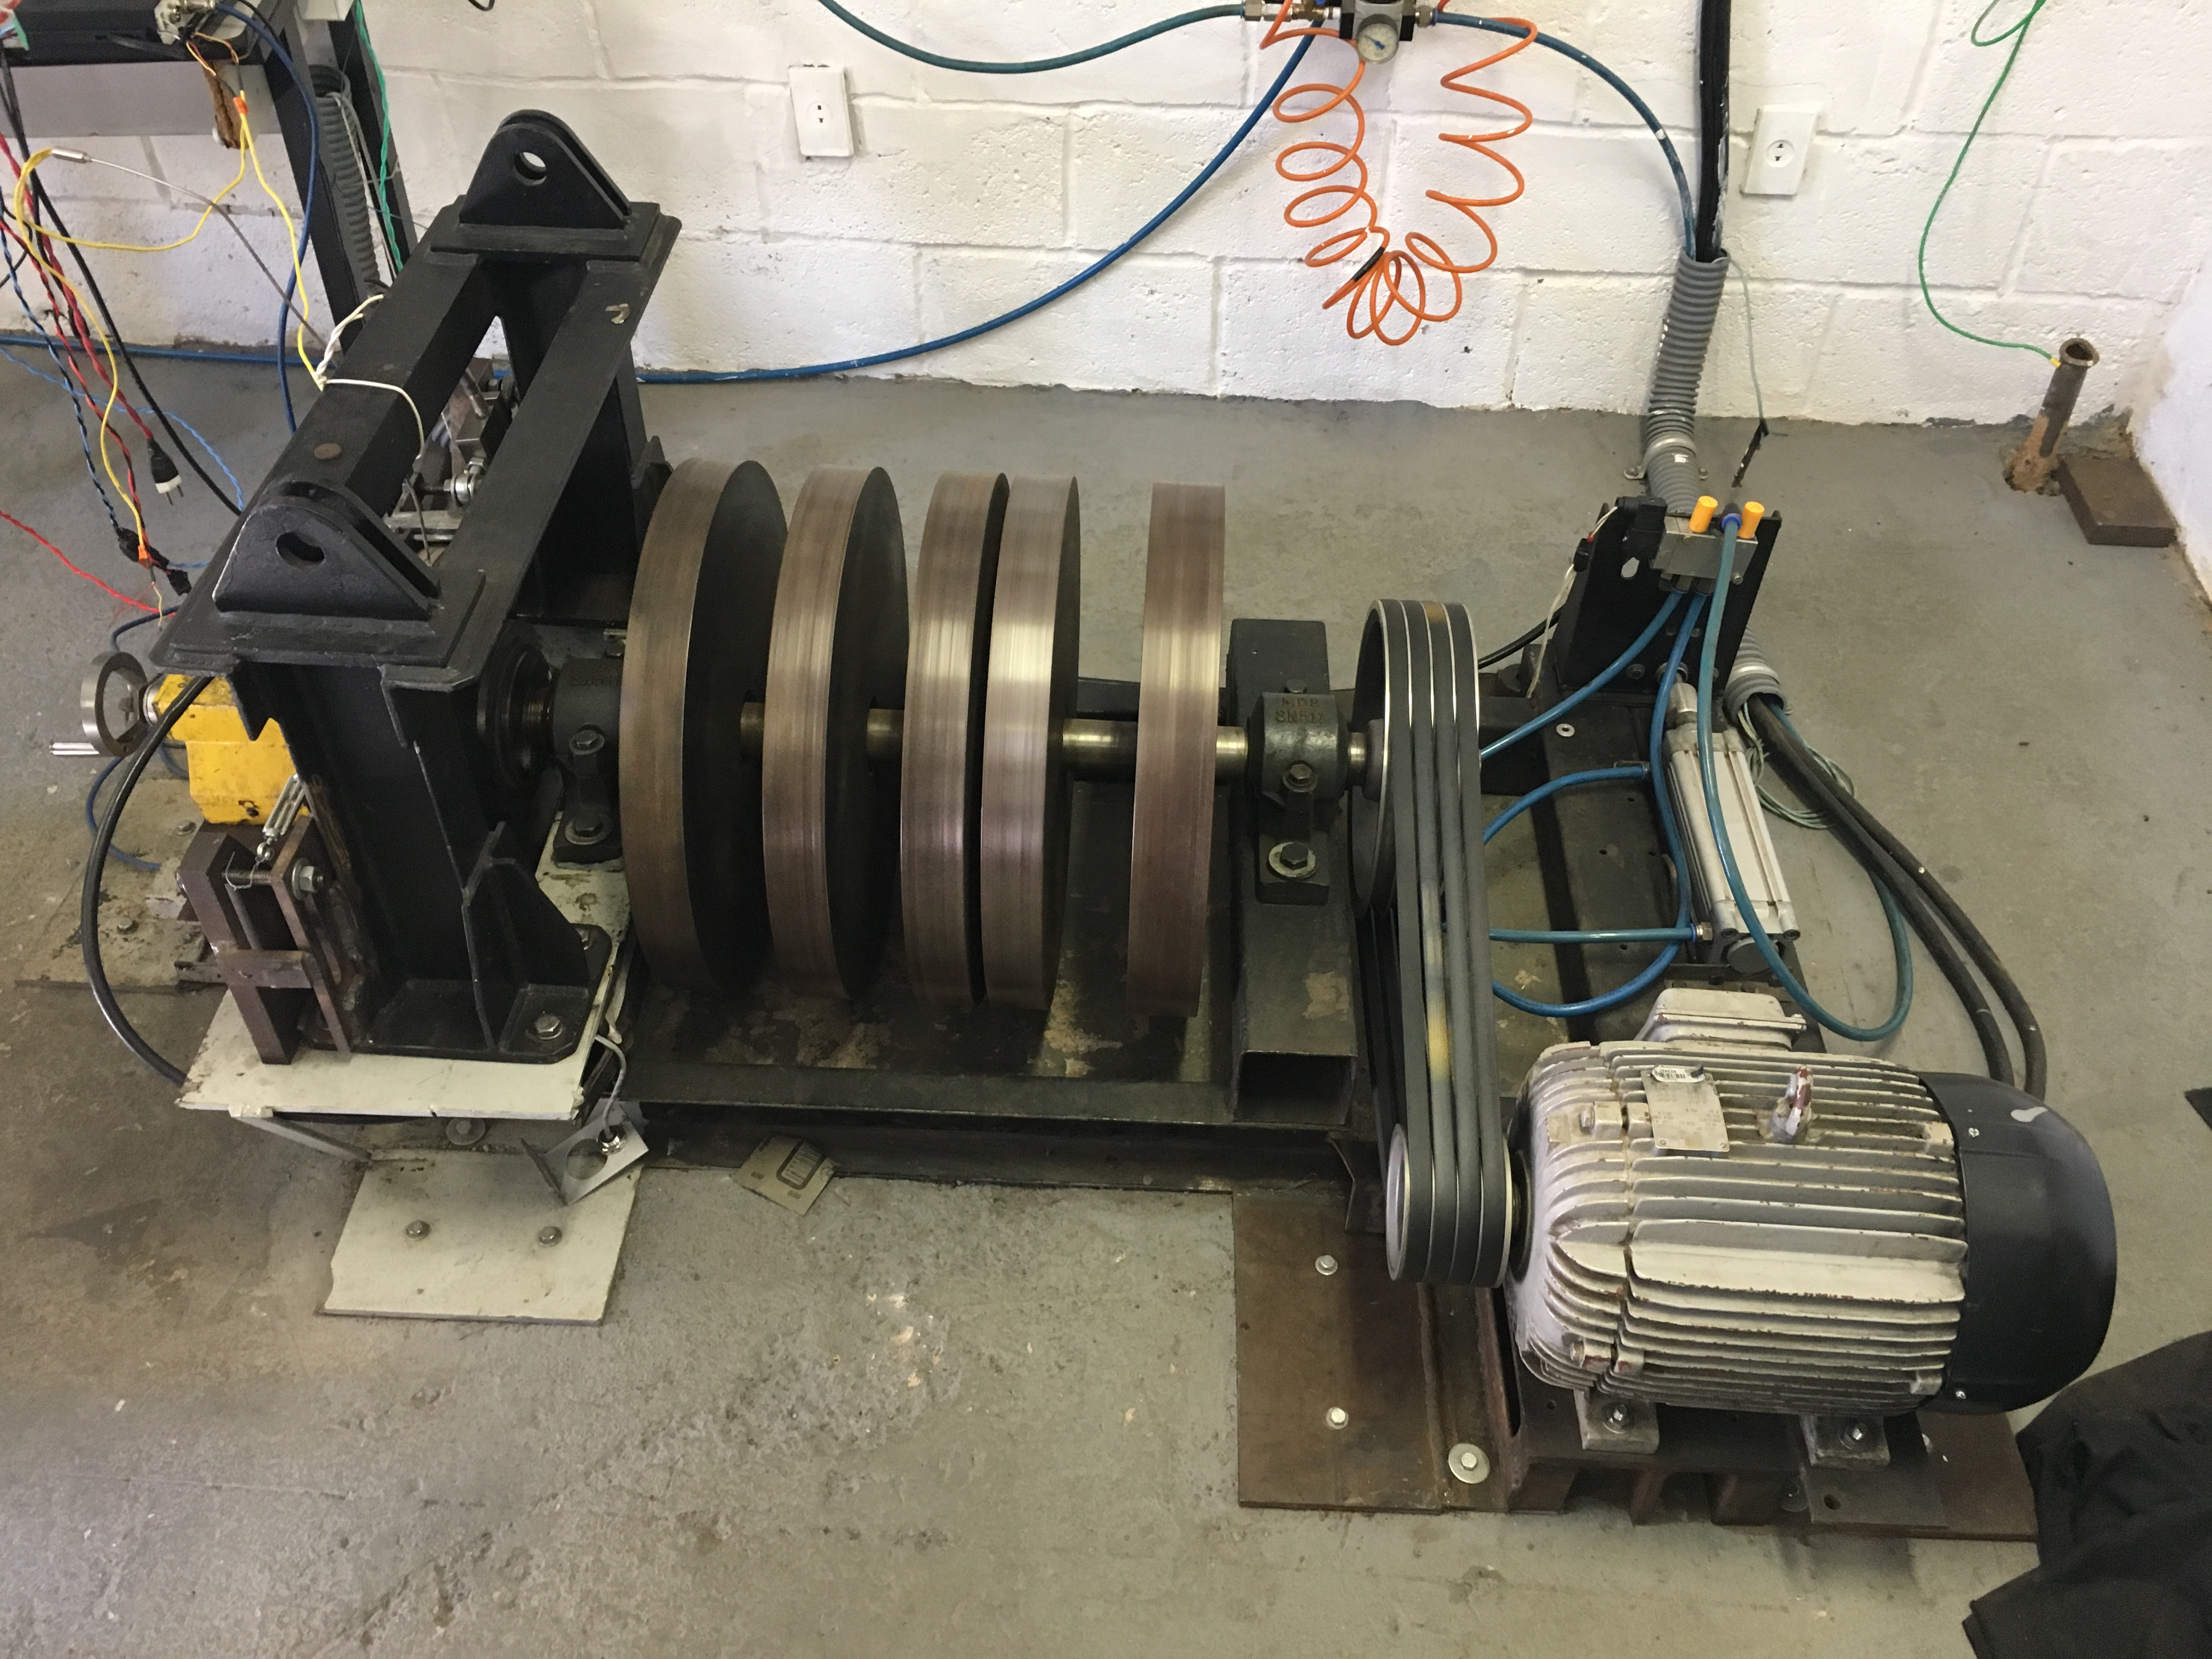
\includegraphics[width=.5\textwidth]{figuras/fig-brake-disc-machine}
			\caption{Brake Disc Machine}
			\label{fig:brake-disc-machine}
		\end{figure}

		\begin{figure}[htbp]
			\centering
			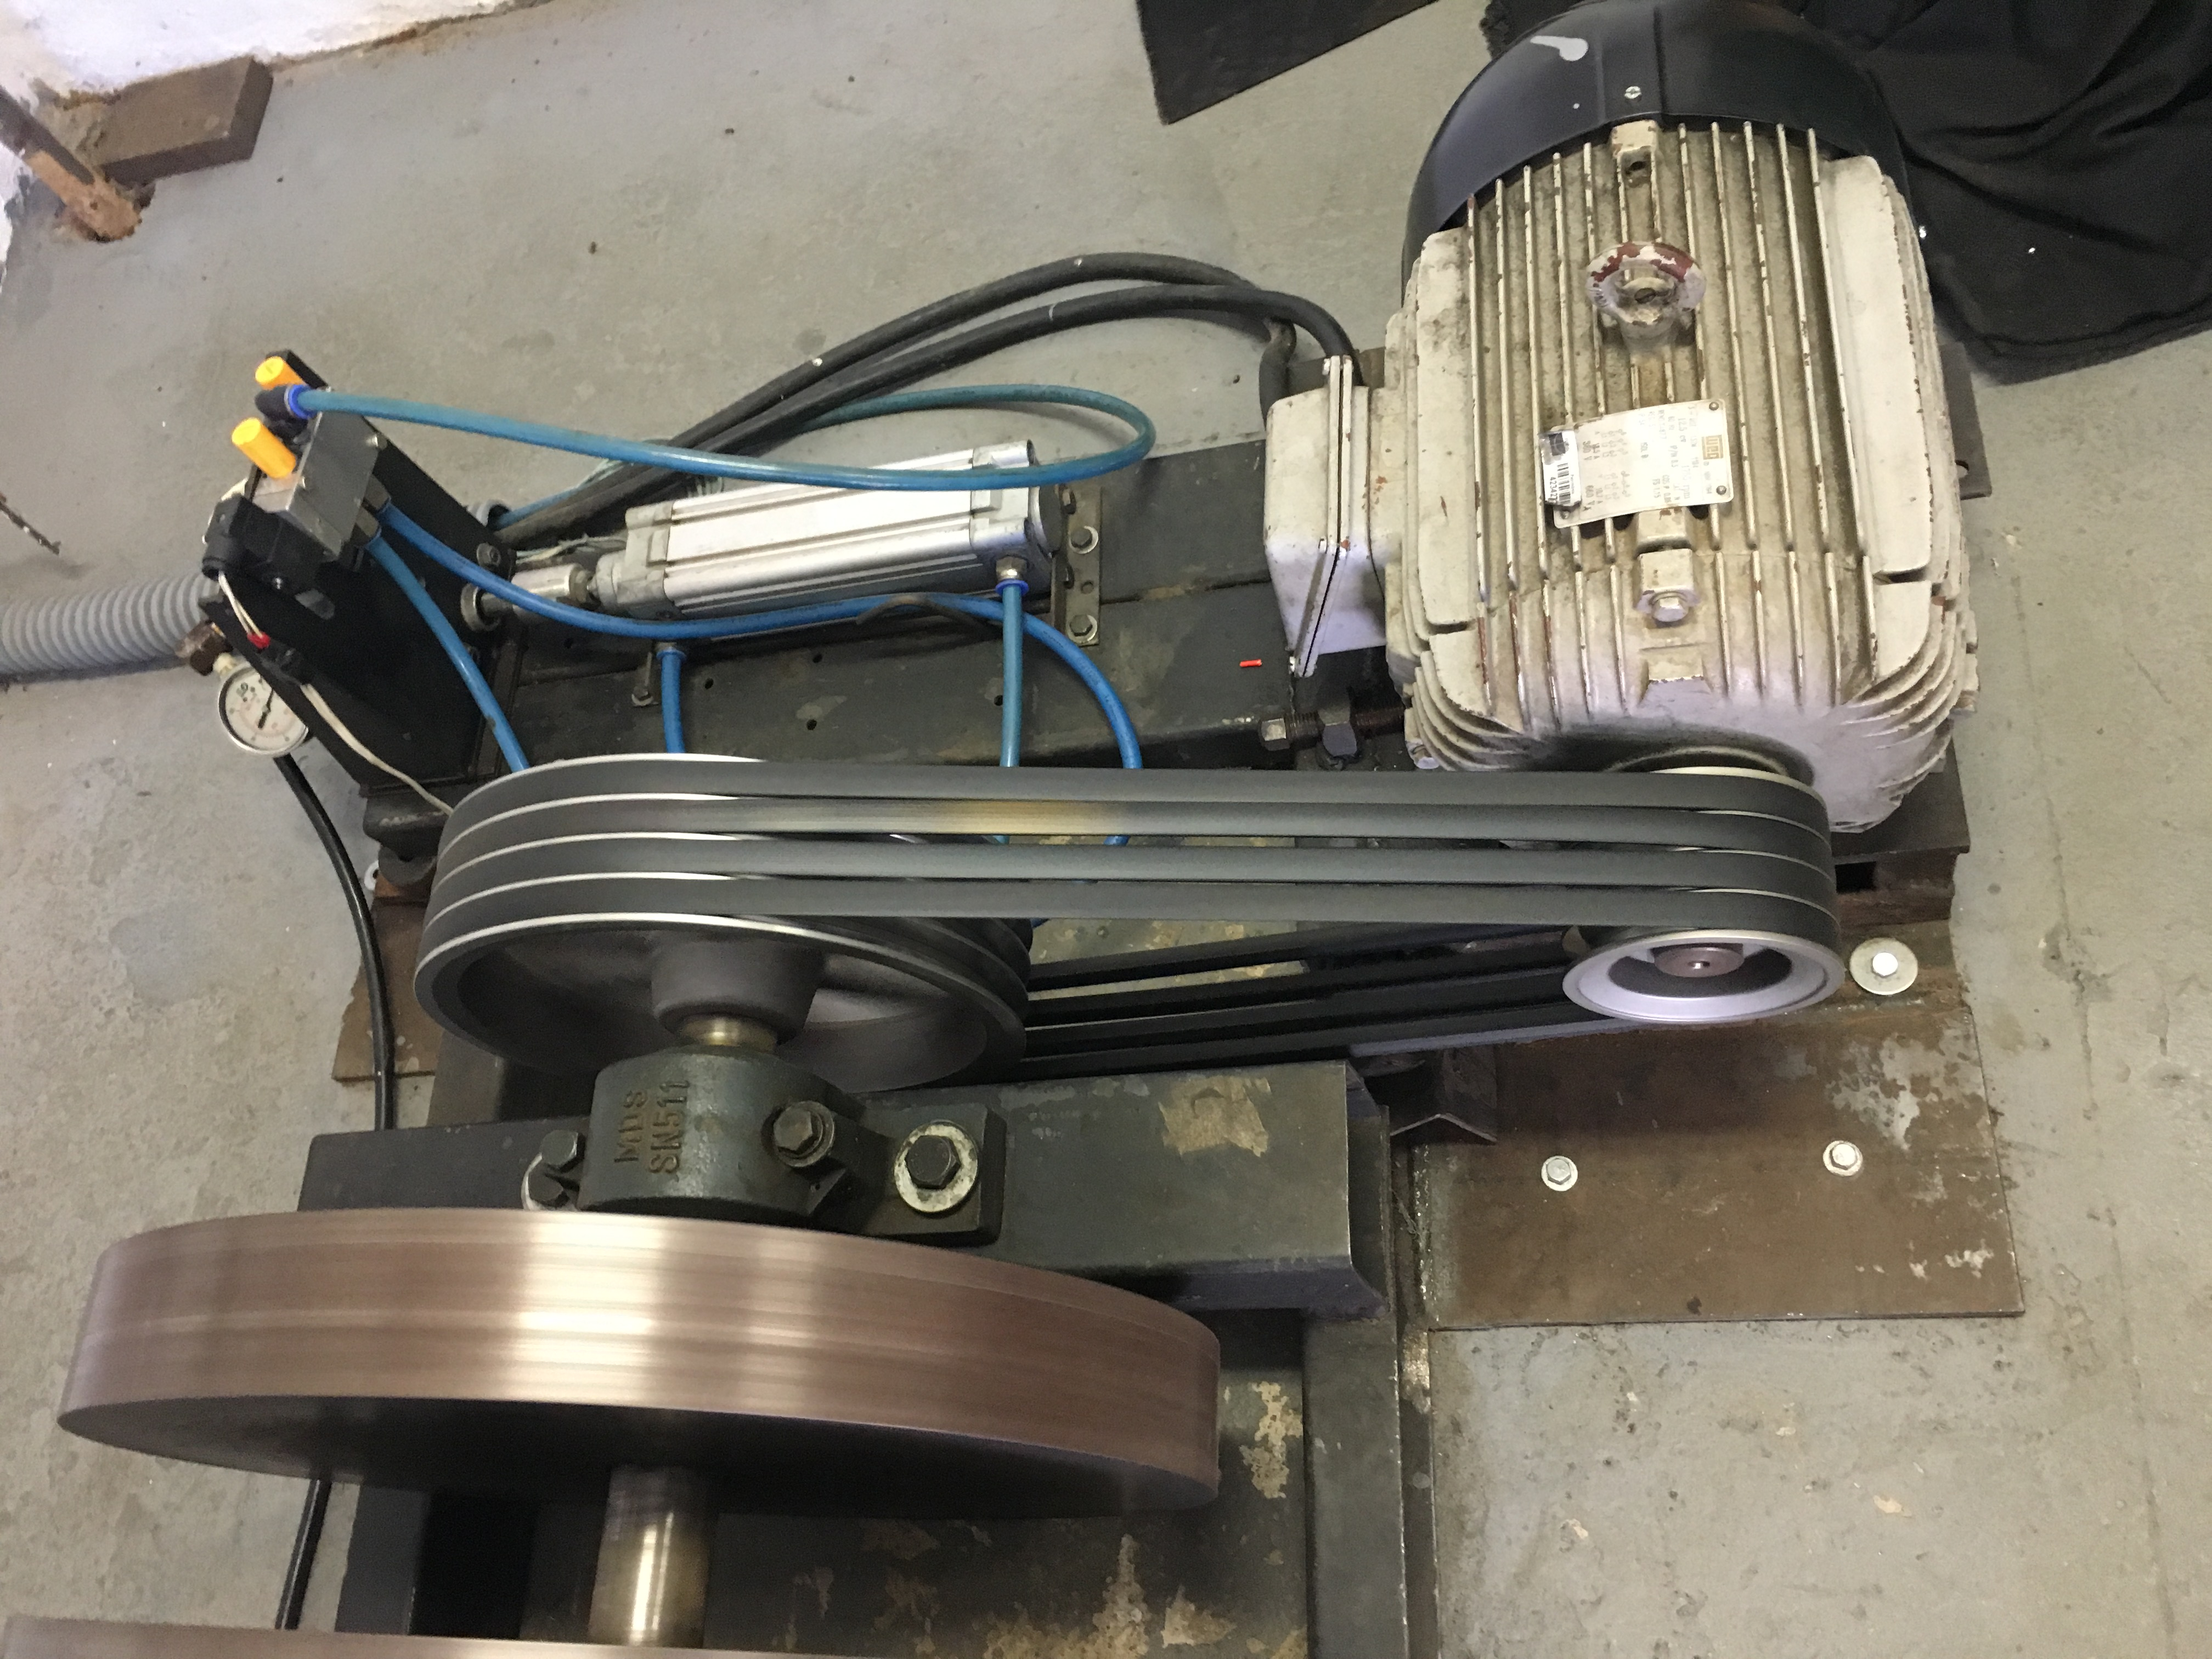
\includegraphics[width=.5\textwidth]{figuras/fig-brake-disc-machine-pulley}
			\caption{Brake Disc Machine Pulley System}
			\label{fig:brake-disc-machine-pulley}
		\end{figure}

		\begin{figure}[htbp]
			\centering
			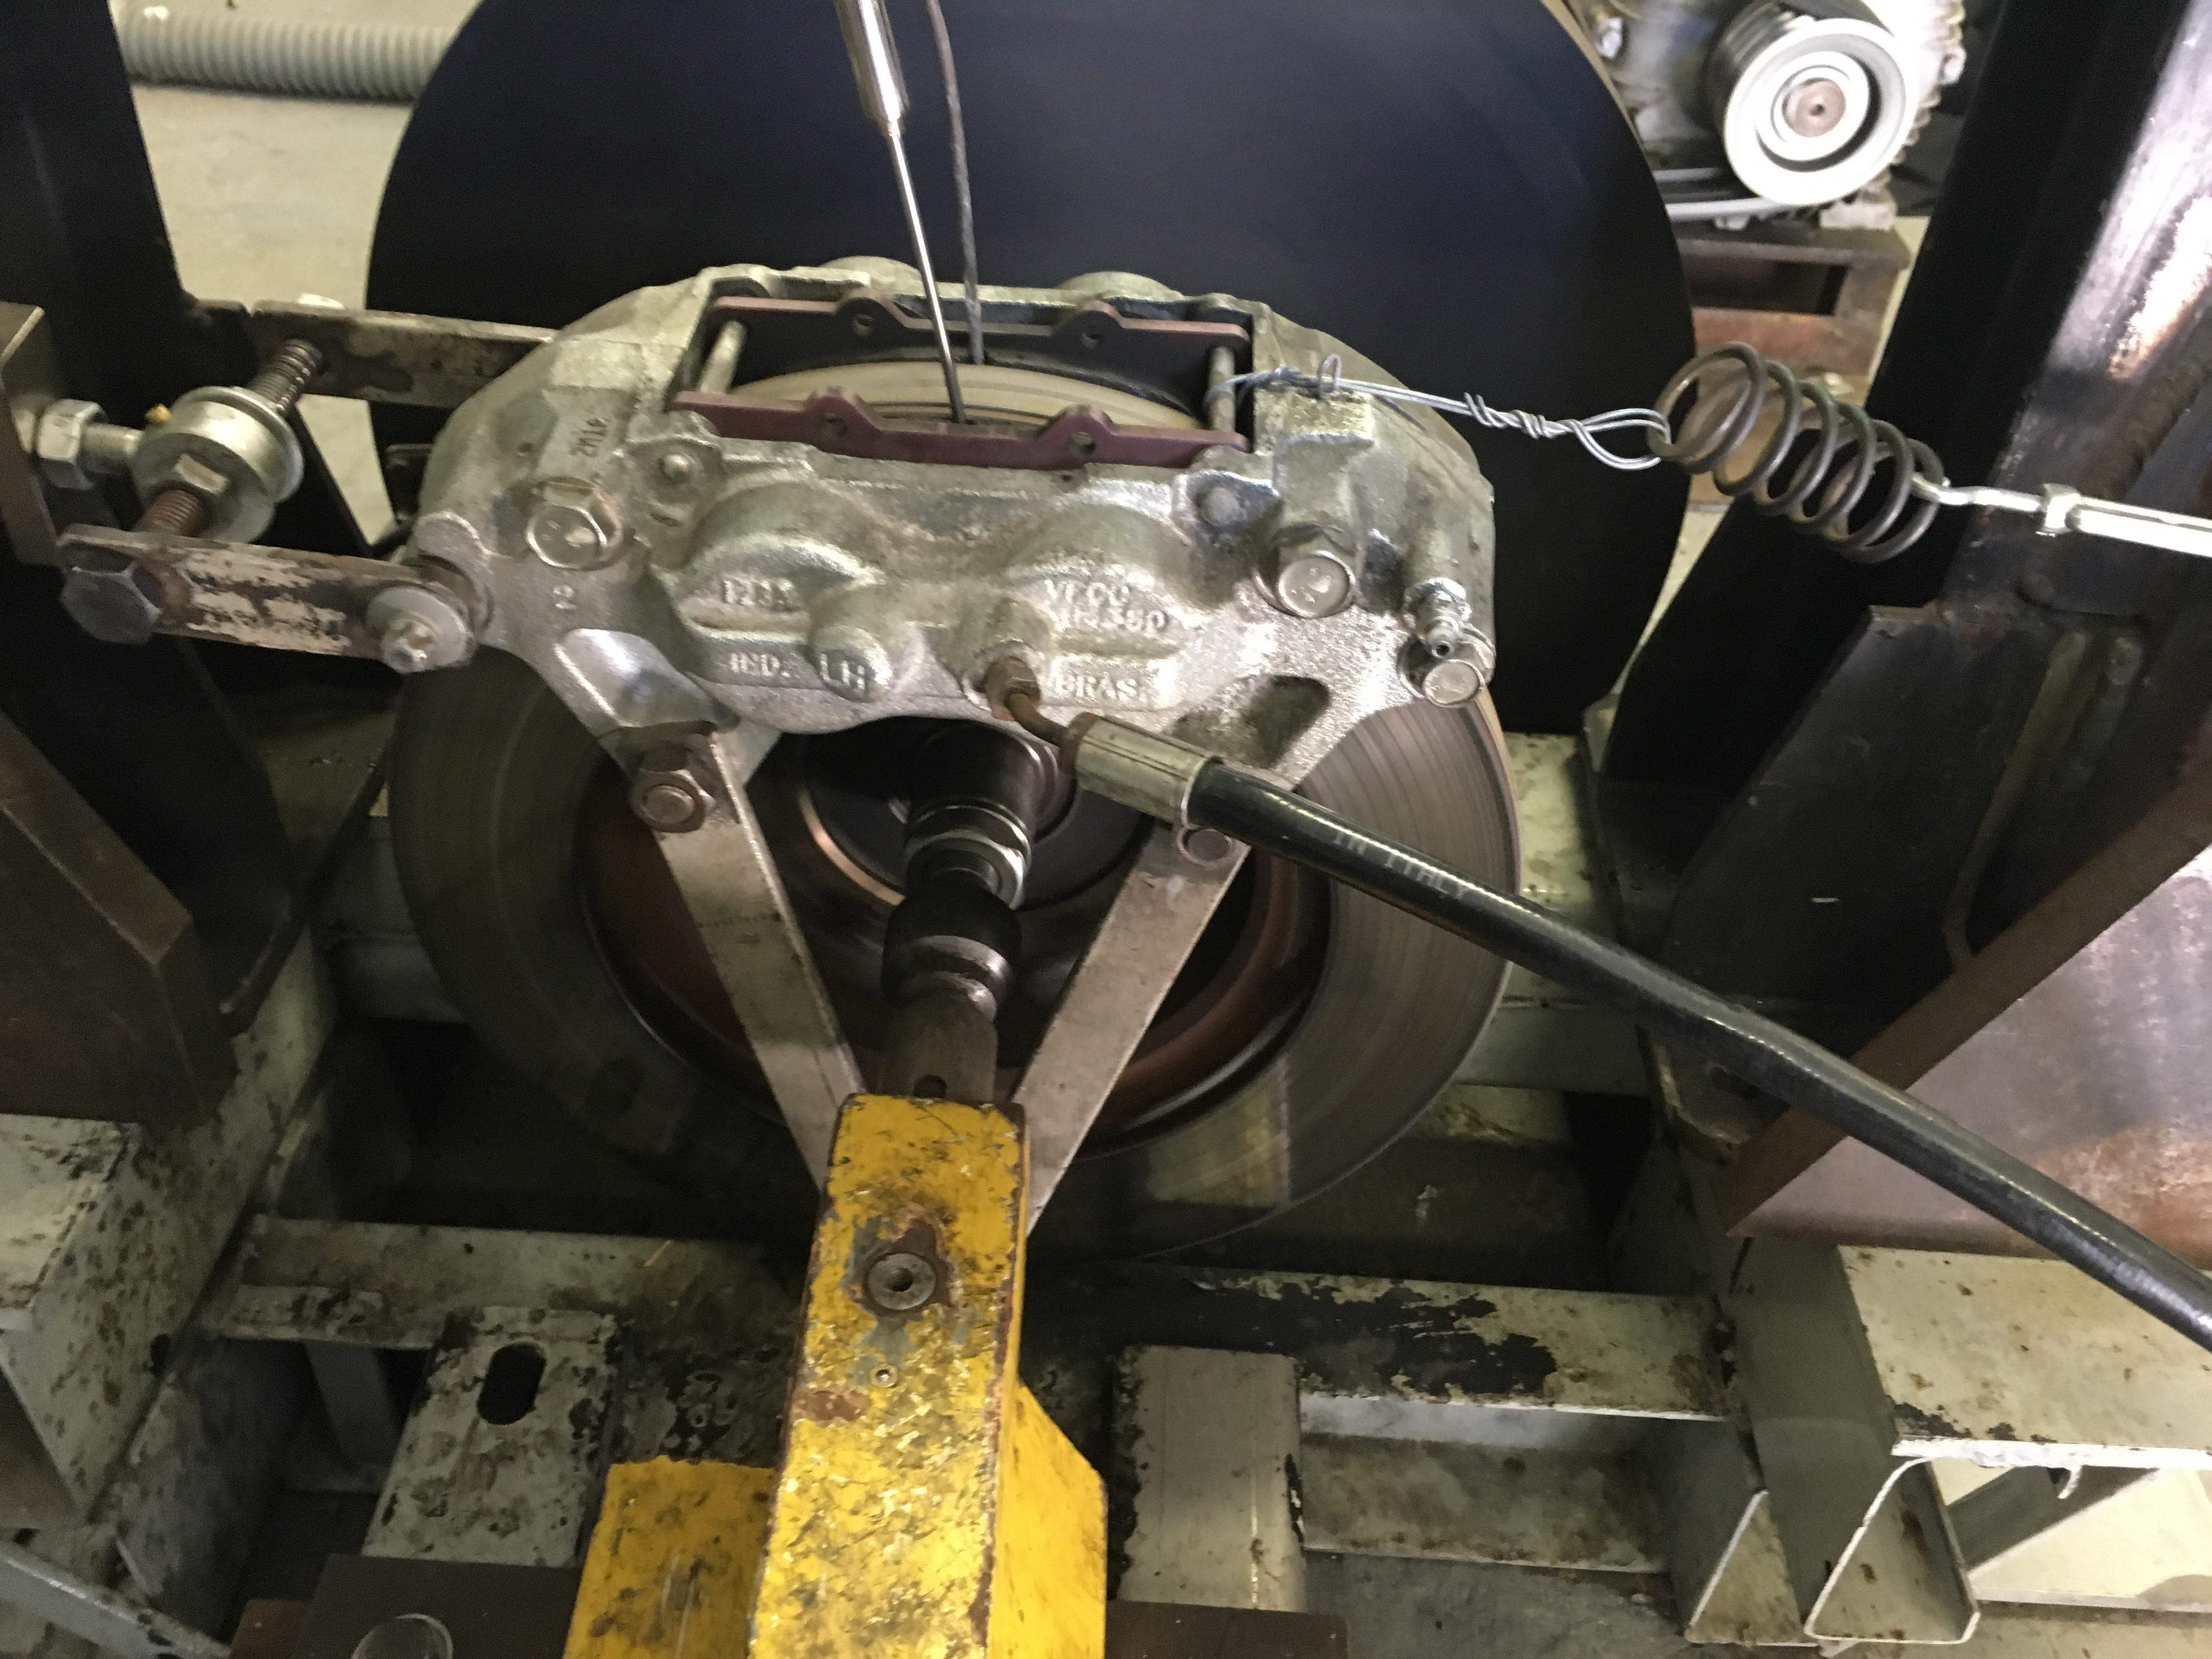
\includegraphics[width=.5\textwidth]{figuras/fig-brake-disc}
			\caption{Brake Disc Arrangment}
			\label{fig:brake-disc}
		\end{figure}
		\par

		The Load Cell used to measure the brake force has a sensibility of 2mV/V and a maximum load of 500kgf, meaning when it is powered with 2V5 (check Section \ref{ssec:load-cell-signal-conditioning}) and submitted to its maximum load the voltage output will be of 5mV. Figure \ref{fig:load-cell-installation-scheme} shows how the load cell can be used to measured the braking force and Figure \ref{fig:load-cell-installed} shows the actual load cell installed on the Brake Disc Machine.

		\begin{figure}[htbp]
			\centering
			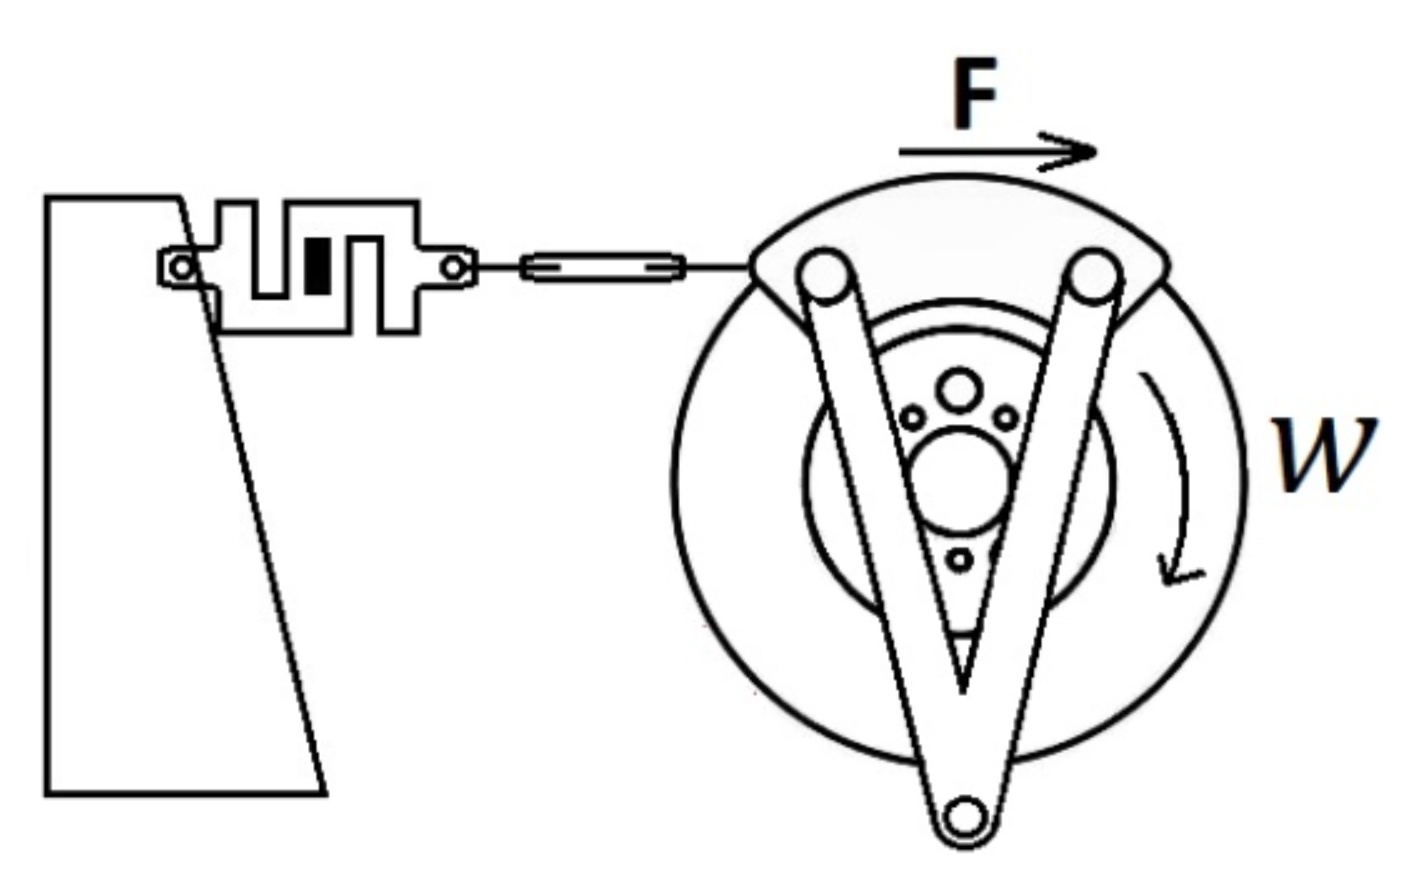
\includegraphics[width=.5\textwidth]{figuras/fig-load-cell-installation-scheme}
			\caption{Load Cell Installation Scheme \cite{caixeta2017}}
			\label{fig:load-cell-installation-scheme}
		\end{figure}

		\begin{figure}[htbp]
			\centering
			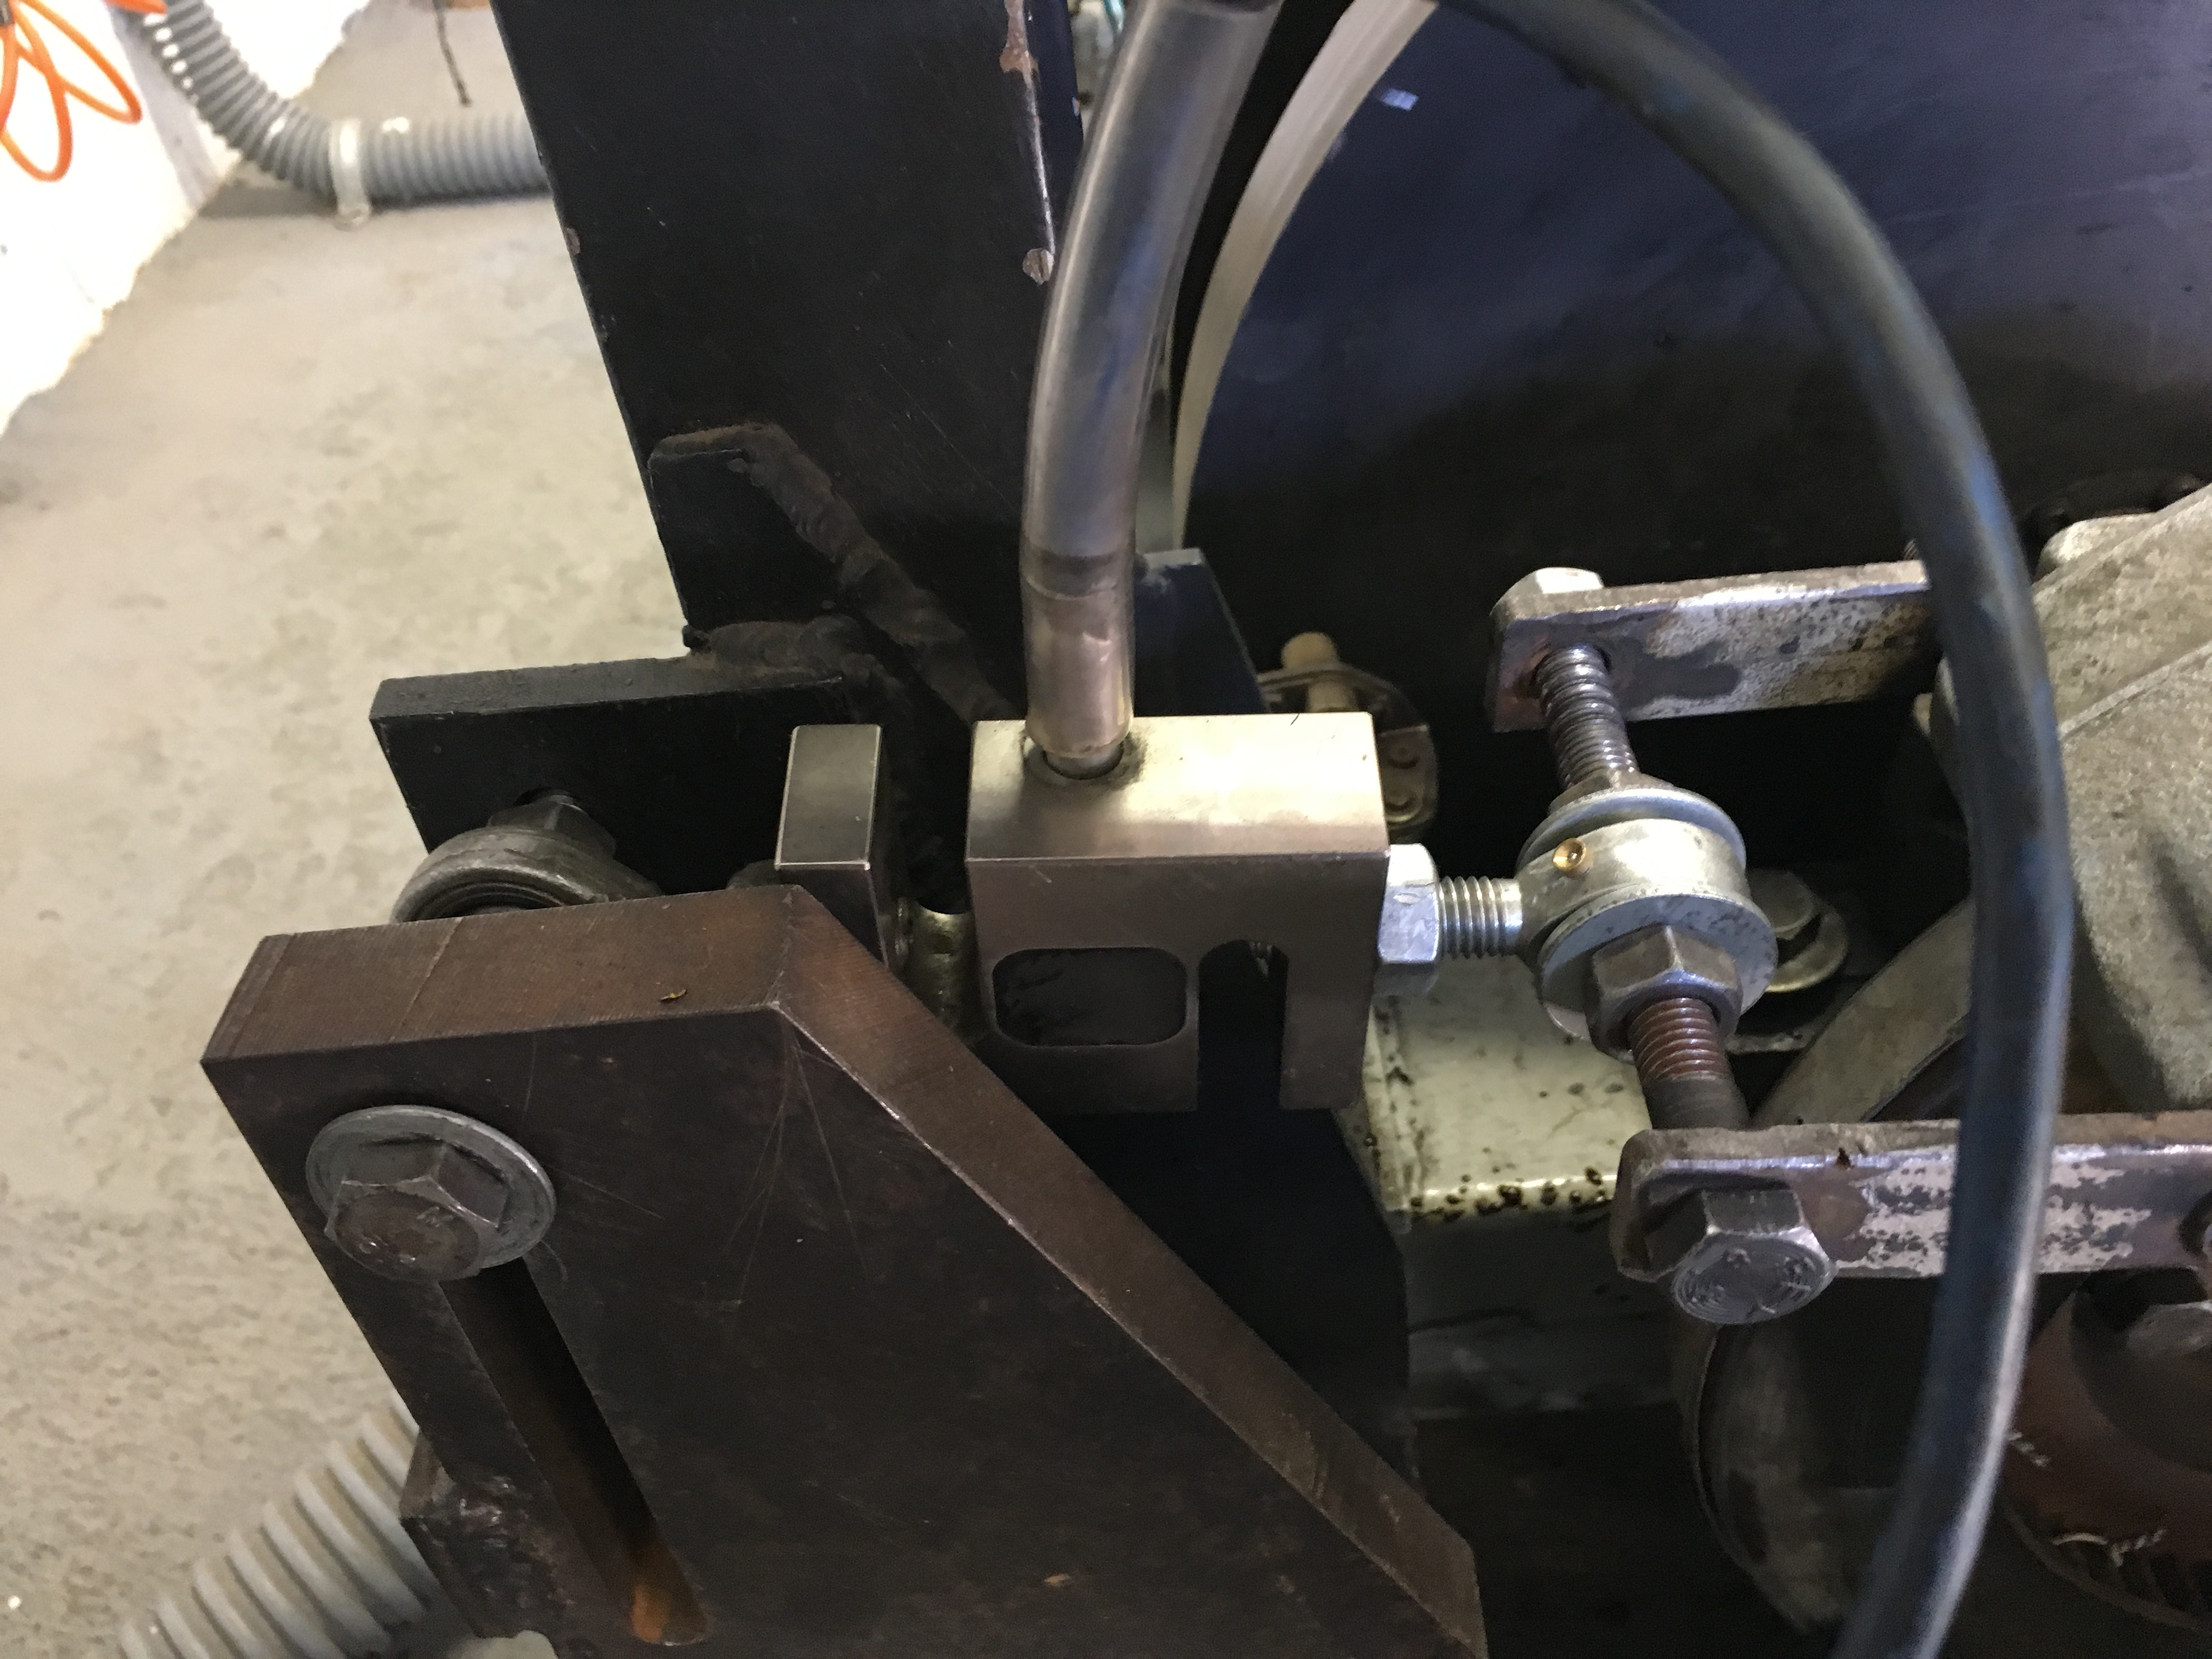
\includegraphics[width=.5\textwidth]{figuras/fig-load-cell-installed}
			\caption{Load Cell Installed}
			\label{fig:load-cell-installed}
		\end{figure}
		\par

		This project uses two generic type K themocouples at each end of the braking disc, as Figure \ref{fig:thermocouple-installation} shows.

		\begin{figure}[htbp]
			\centering
			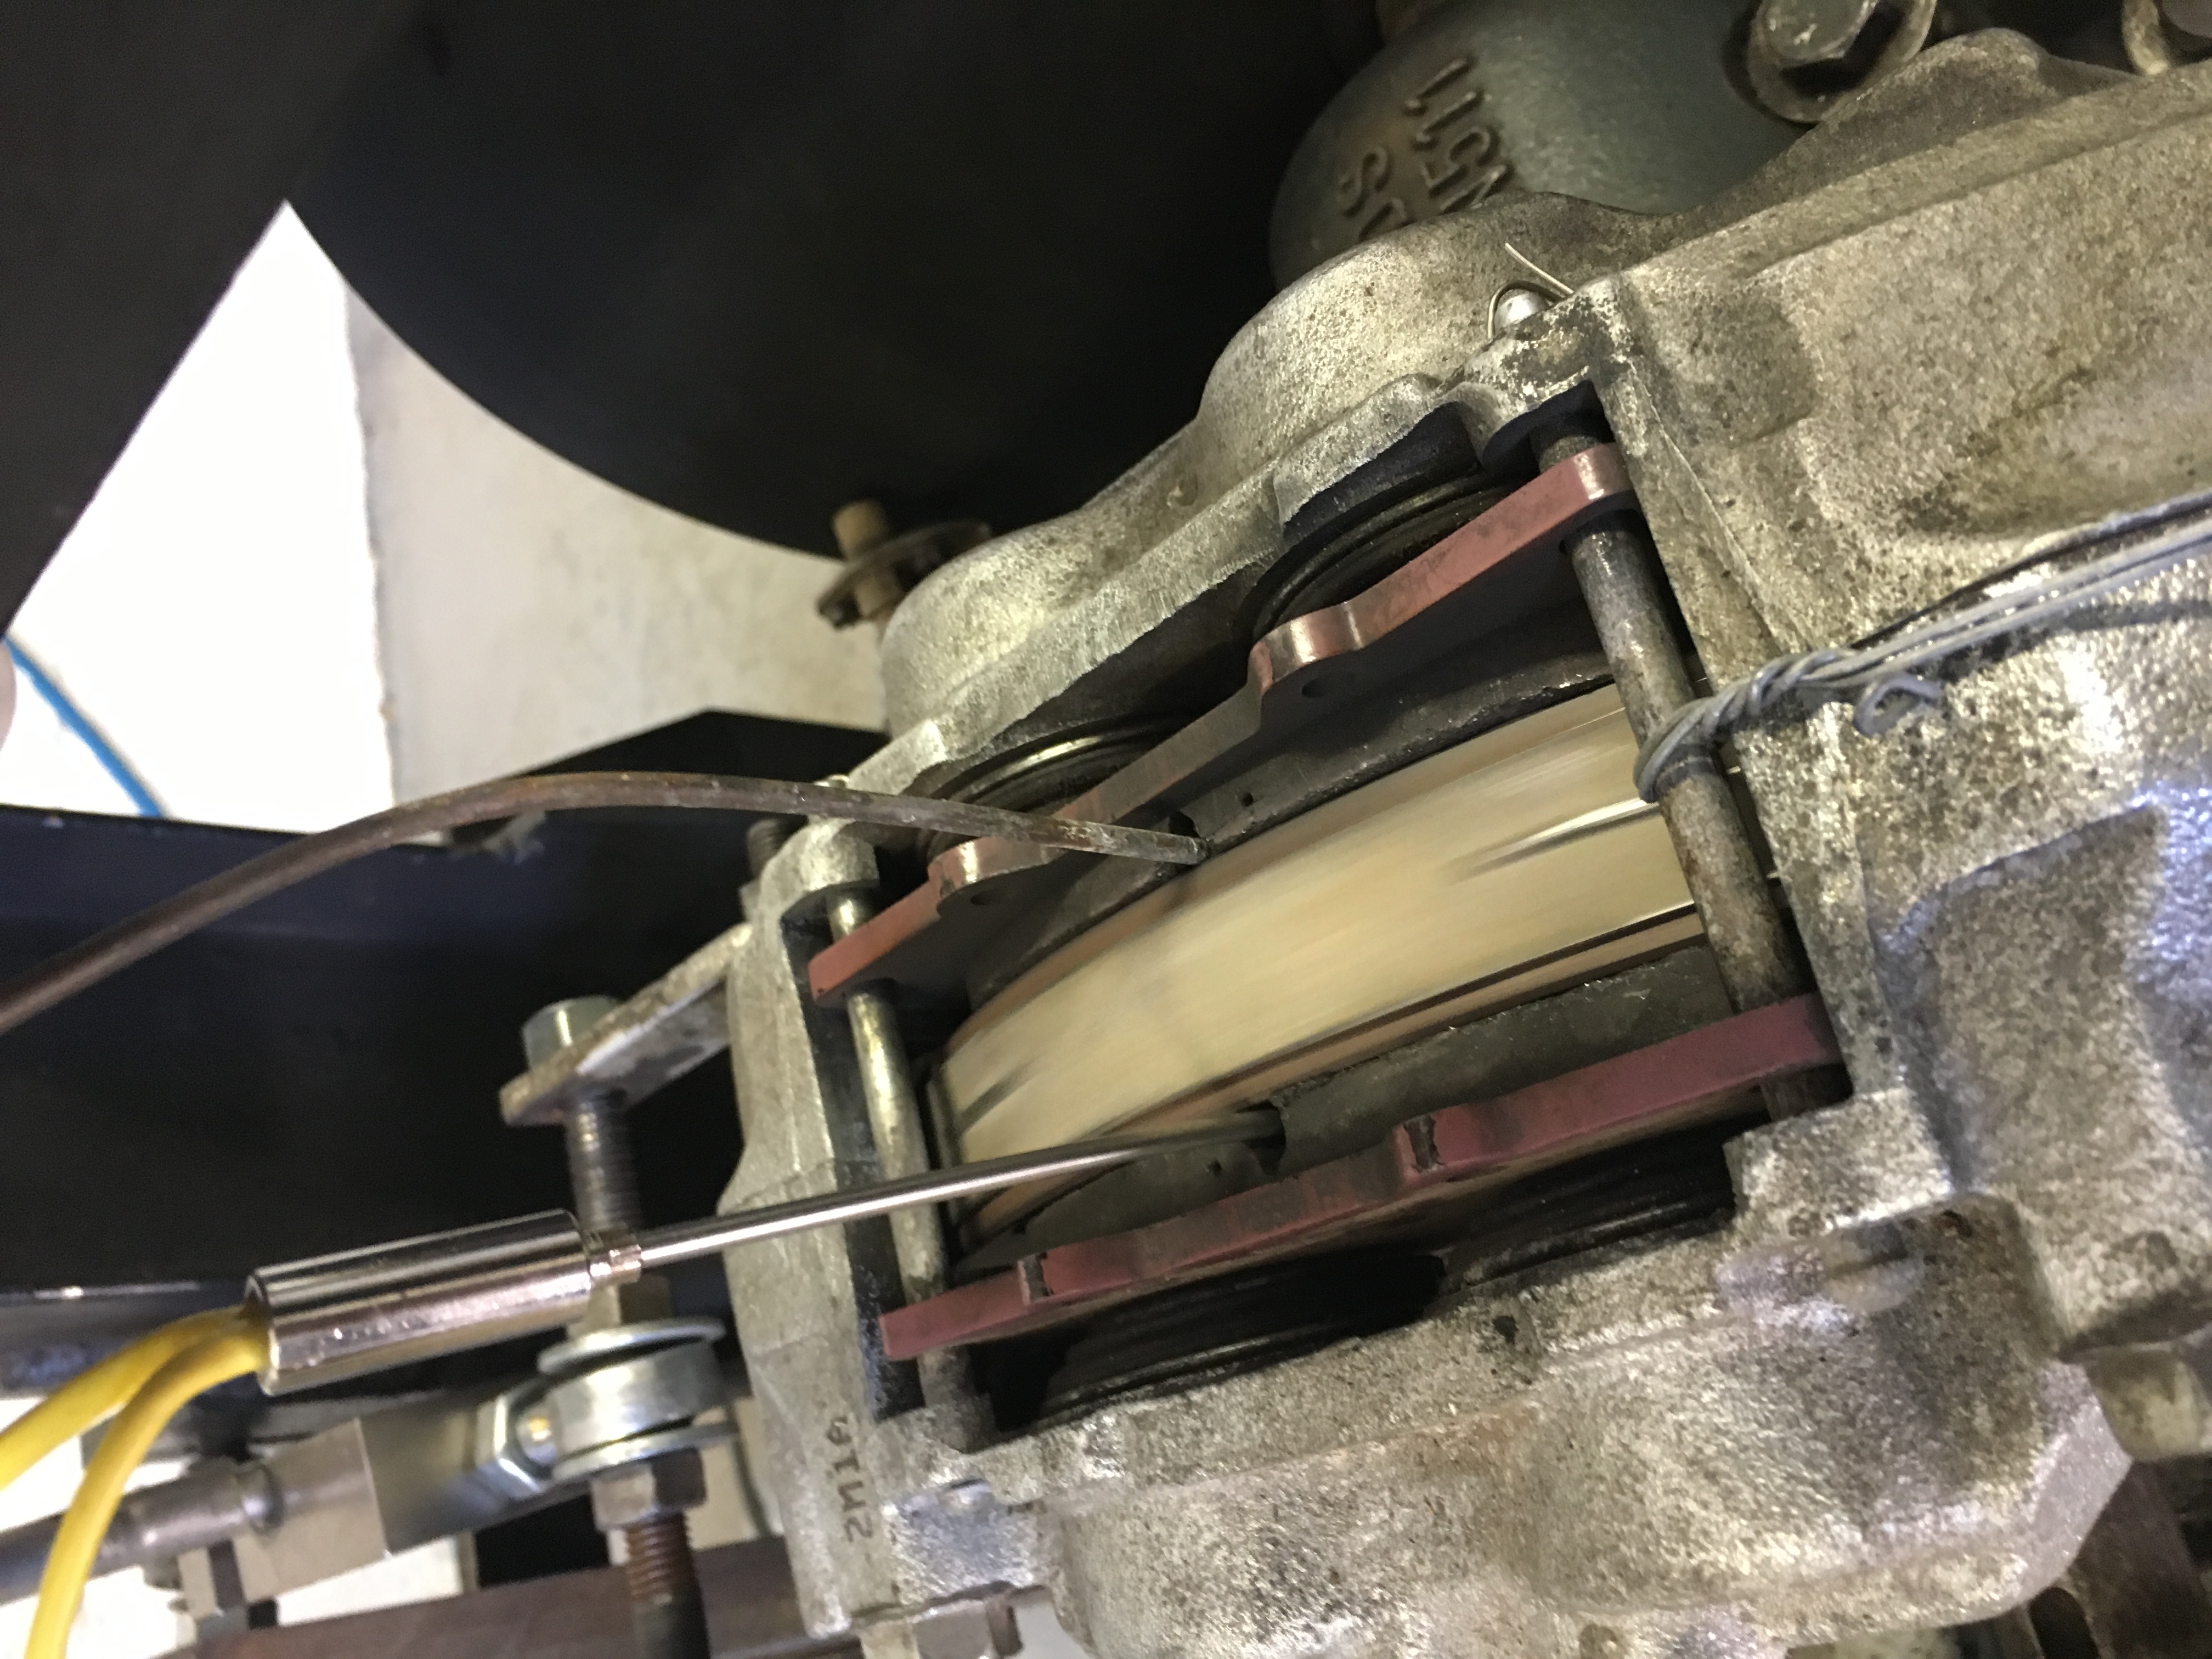
\includegraphics[width=.5\textwidth, angle=270]{figuras/fig-thermocouple-installation}
			\caption{Thermocouples Installed}
			\label{fig:thermocouple-installation}
		\end{figure}
		\par

		This project also includes a generic Crankshaft Position Sensor, to enhance the CKP signal amplitude six small magnets were placed around the inertial disc that the CKP is perpendicular mounted to, the only important consideration when doing this is that the CKP will actualy measure a frequency six times higher than the actual rotation frequency of the axel. Figure \ref{fig:ckp-installed} shows how the CKP sensor was placed.

		\begin{figure}[htbp]
			\centering
			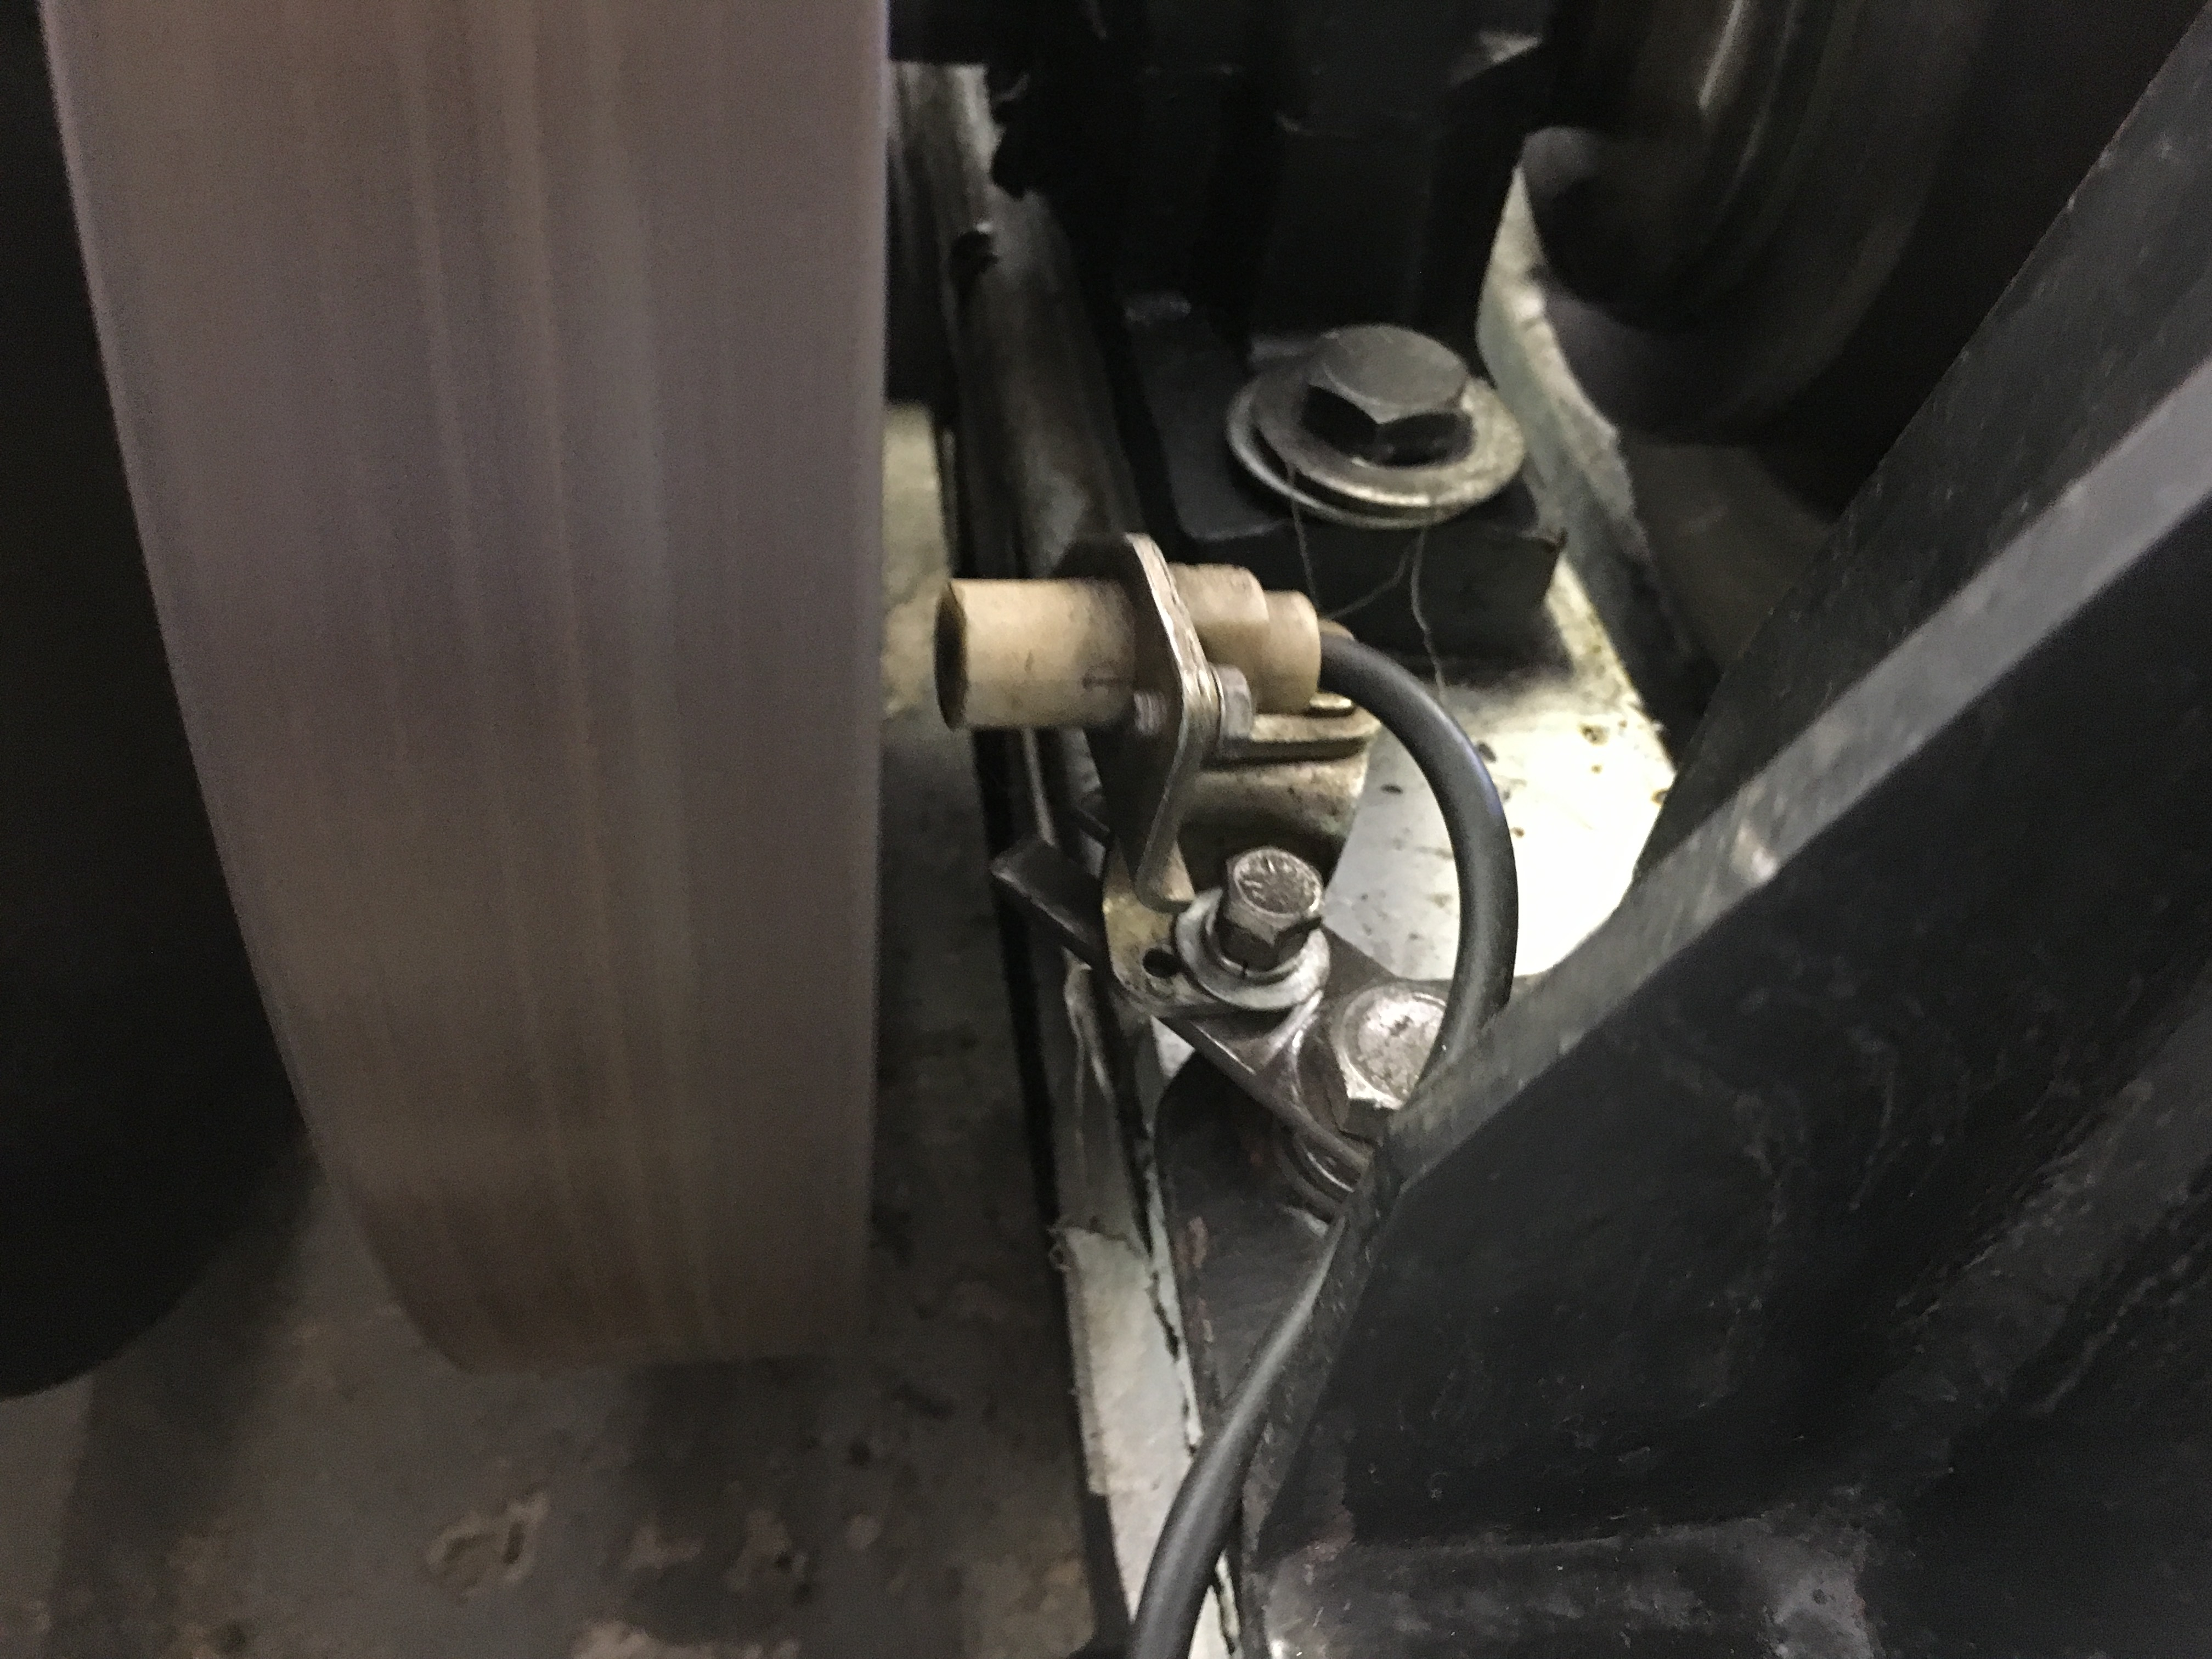
\includegraphics[width=.5\textwidth]{figuras/fig-ckp-installed}
			\caption{CKP installed}
			\label{fig:ckp-installed}
		\end{figure}
		\par

		Additional materials used for the test are the developed hardware and the laptop used to run the test.